\lessonsection{Bài tập phản xạ PX1--PX6}
\pxtitle{PX1. Phản ứng chạy hai chiều: vì sao chất đầu không bao giờ hết}
\begin{readingpassage}[Ngữ liệu lạ]
Cho 3,0 mol khí HI vào một bình kín dung tích 10 L, giữ ở 445 °C. Sau 1 giờ, 1 ngày rồi 1 tuần, kết quả phân tích khí trong bình luôn giống nhau: 2,4 mol HI; 0,3 mol H$_{2}$ và 0,3 mol I$_{2}$.

Ở một bình kín khác cùng dung tích và cùng nhiệt độ, người ta cho 1,5 mol H$_{2}$ và 1,5 mol I$_{2}$, không có HI. Sau một thời gian, trong bình đo được 0,3 mol H$_{2}$.

Trong một thí nghiệm thứ ba, đốt cháy 1 mol CH$_{4}$ trong lượng O$_{2}$ dư. Sau phản ứng, trong bình không còn CH$_{4}$.

\end{readingpassage}
\Needspace{12\baselineskip}
\qhead
\begin{enumerate}[label={}, leftmargin=0.5em, itemsep=4pt]
\Needspace{8\baselineskip}
\item \textbf{(1)} Viết phương trình hai phản ứng xảy ra đồng thời trong bình thứ nhất, rồi gộp lại thành một phương trình phản ứng thuận nghịch. \answerlines{4}
\Needspace{8\baselineskip}
\item \textbf{(2)} Tính phần trăm số mol HI đã bị phân hủy trong bình thứ nhất. \answerlines{4}
\Needspace{8\baselineskip}
\item \textbf{(3)} Vì sao chờ đến 1 tuần mà HI vẫn không phân hủy hết? \answerlines{4}
\Needspace{10\baselineskip}
\item \textbf{(4)} Trong bình thứ hai, tính số mol I$_{2}$ và HI tại thời điểm đo được 0,3 mol H$_{2}$. So sánh thành phần khí này với bình thứ nhất và rút ra nhận xét. \answerlines{6}
\Needspace{8\baselineskip}
\item \textbf{(5)} Phản ứng đốt cháy CH$_{4}$ khác phản ứng trong hai bình trên ở điểm nào? \answerlines{4}
\end{enumerate}
\pxtitle{PX2. Lượng chất đứng yên nhưng phản ứng vẫn chạy (cân bằng động)}
\begin{readingpassage}[Ngữ liệu lạ]
Cho 1,00 mol N$_{2}$ và 3,00 mol H$_{2}$ vào bình kín dung tích 1 L có xúc tác, giữ ở nhiệt độ không đổi. Số mol các chất được đo định kì và ghi trong Bảng 1.1.

\Needspace{5cm}
\tablecaption{1.1}{Số mol các chất trong bình theo thời gian.}
{\small
\begin{center}
\renewcommand{\arraystretch}{1.3}
\begin{tabular}{|c|c|c|c|c|c|c|}
\hline
\rowcolor{pastelBlue}
\textbf{Thời gian (phút)} & \textbf{0} & \textbf{10} & \textbf{20} & \textbf{30} & \textbf{40} & \textbf{50} \\
\hline
Số mol N$_{2}$ & 1,00 & 0,80 & 0,68 & 0,62 & 0,60 & 0,60 \\
\hline
Số mol H$_{2}$ & 3,00 & 2,40 & 2,04 & 1,86 & 1,80 & 1,80 \\
\hline
Số mol NH$_{3}$ & 0 & 0,40 & 0,64 & 0,76 & 0,80 & 0,80 \\
\hline
\end{tabular}
\end{center}
}
Ở phút thứ 50, người ta rút toàn bộ H$_{2}$ ra và thay bằng đúng 1,80 mol D$_{2}$ (D là đồng vị nặng của hydrogen, tính chất hóa học gần như giống hệt H). Một thời gian sau, tổng số mol N$_{2}$, khí hydrogen và ammonia vẫn là 0,60 mol, 1,80 mol và 0,80 mol, nhưng trong bình xuất hiện các phân tử NH$_{2}$D, NHD$_{2}$, ND$_{3}$ và cả khí HD.

\end{readingpassage}
\Needspace{12\baselineskip}
\qhead
\begin{enumerate}[label={}, leftmargin=0.5em, itemsep=4pt]
\Needspace{8\baselineskip}
\item \textbf{(1)} Viết phương trình phản ứng. Từ phút thứ mấy hệ bắt đầu ở trạng thái cân bằng? Dựa vào đâu? \answerlines{4}
\Needspace{10\baselineskip}
\item \textbf{(2)} Tính tốc độ tăng số mol NH$_{3}$ trung bình (mol/phút) trong khoảng 0 đến 10 phút và trong khoảng 30 đến 40 phút. Giải thích vì sao hai giá trị chênh nhau nhiều như vậy. \answerlines{6}
\Needspace{10\baselineskip}
\item \textbf{(3)} Bạn A cho rằng: ``Từ phút 40, phản ứng đã dừng vì số mol không đổi''. Thí nghiệm thay H$_{2}$ bằng D$_{2}$ ủng hộ hay bác bỏ ý kiến này? Giải thích. \answerlines{6}
\Needspace{10\baselineskip}
\item \textbf{(4)} Mô tả dạng đồ thị v(thuận) và v(nghịch) theo thời gian từ phút 0 đến phút 50. \answerlines{6}
\Needspace{8\baselineskip}
\item \textbf{(5)} Tại phút thứ 50, v(thuận) và v(nghịch) có bằng 0 không? So sánh hai tốc độ này. \answerlines{4}
\end{enumerate}
\pxtitle{PX3. Viết Kc: chất nào vào, chất nào bỏ ra}
\begin{readingpassage}[Ngữ liệu lạ]
Cho bốn phản ứng thuận nghịch:

(a) 2SO$_{2}$(g) + O$_{2}$(g) $\rightleftharpoons$ 2SO$_{3}$(g)

(b) CaCO$_{3}$(s) $\rightleftharpoons$ CaO(s) + CO$_{2}$(g)

(c) C(s) + H$_{2}$O(g) $\rightleftharpoons$ CO(g) + H$_{2}$(g)

(d) Fe$_{3}$O$_{4}$(s) + 4H$_{2}$(g) $\rightleftharpoons$ 3Fe(s) + 4H$_{2}$O(g)

Ở 800 °C, phản ứng (b) có Kc $\approx$ 0,0025. Một chất rắn nguyên chất có khối lượng riêng xác định, nên số mol chất trong mỗi lít chất rắn là một hằng số, không phụ thuộc ta có nhiều hay ít chất rắn đó.

Trong công nghiệp, vôi sống được sản xuất trong lò nung vôi (Hình 1). Đá vôi đổ vào từ đỉnh lò, được nung nóng ở khoảng 900 °C đến 1000 °C; khí thải chứa CO$_{2}$ được quạt hút ra ngoài liên tục, vôi sống lấy ra ở đáy lò.

\begin{center}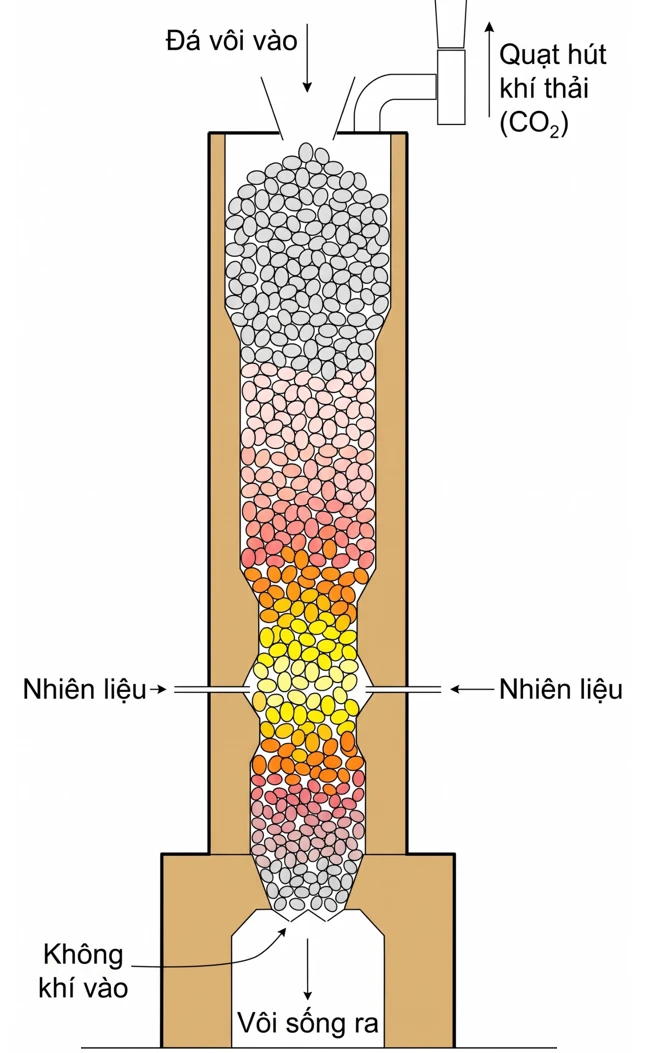
\includegraphics[width=0.45\textwidth,height=9cm,keepaspectratio]{image/lo_nung_voi.png}\end{center}
\figcaption{1}{Lò nung vôi: quạt hút CO$_{2}$ để CaCO$_{3}$ phân hủy gần hết (Nguồn: Wikipedia, ``Lime kiln'' (Việt hóa))}
\end{readingpassage}
\Needspace{16\baselineskip}
\qhead
\begin{enumerate}[label={}, leftmargin=0.5em, itemsep=4pt]
\Needspace{12\baselineskip}
\item \textbf{(1)} Viết biểu thức Kc của bốn phản ứng (a), (b), (c), (d). \answerlines{8}
\Needspace{8\baselineskip}
\item \textbf{(2)} Dùng thông tin trong ngữ liệu, giải thích vì sao nồng độ chất rắn không được đưa vào biểu thức Kc. \answerlines{4}
\Needspace{10\baselineskip}
\item \textbf{(3)} Một bình kín 10 L chứa một lượng lớn CaCO$_{3}$, giữ ở 800 °C đến khi cân bằng. Tính số mol CO$_{2}$ trong bình. Nếu ban đầu cho lượng CaCO$_{3}$ gấp đôi (vẫn dư) thì số mol CO$_{2}$ lúc cân bằng thay đổi thế nào? \answerlines{6}
\Needspace{10\baselineskip}
\item \textbf{(4)} Trong lò nung vôi (Hình 1), CaCO$_{3}$ bị phân hủy gần hết thành vôi sống, còn trong bình kín ở ý (3) thì chỉ 0,025 mol CaCO$_{3}$ bị phân hủy. Dựa vào biểu thức Kc của phản ứng (b), giải thích vai trò của quạt hút. \answerlines{6}
\Needspace{8\baselineskip}
\item \textbf{(5)} Ở một nhiệt độ, phản ứng (a) có Kc = K. Viết biểu thức Kc của phản ứng 2SO$_{3}$(g) $\rightleftharpoons$ 2SO$_{2}$(g) + O$_{2}$(g) và tính giá trị theo K. \answerlines{4}
\end{enumerate}
\pxtitle{PX4. Tính Kc và nồng độ lúc cân bằng bằng bảng ICE}
\begin{readingpassage}[Ngữ liệu lạ]
Ở nhiệt độ T, khí PCl$_{5}$ phân hủy theo phản ứng thuận nghịch: PCl$_{5}$(g) $\rightleftharpoons$ PCl$_{3}$(g) + Cl$_{2}$(g).

Thí nghiệm 1: cho 1,0 mol PCl$_{5}$ vào bình kín 2 L. Khi cân bằng, trong bình còn 0,5 mol PCl$_{5}$.

Thí nghiệm 2: cho 3,0 mol PCl$_{5}$ vào bình kín 2 L, cùng nhiệt độ T.

Ở nhiệt độ T$'$, phản ứng CO(g) + H$_{2}$O(g) $\rightleftharpoons$ CO$_{2}$(g) + H$_{2}$(g) có Kc = 4.

\end{readingpassage}
\Needspace{16\baselineskip}
\qhead
\begin{enumerate}[label={}, leftmargin=0.5em, itemsep=4pt]
\Needspace{12\baselineskip}
\item \textbf{(1)} Lập bảng ICE cho thí nghiệm 1 và tính Kc của phản ứng phân hủy PCl$_{5}$ ở nhiệt độ T. \answerlines{8}
\Needspace{14\baselineskip}
\item \textbf{(2)} Bạn B cho rằng ở thí nghiệm 2, lượng PCl$_{5}$ gấp ba nên Kc cũng gấp ba. Tính nồng độ các chất lúc cân bằng ở thí nghiệm 2 và nhận xét ý kiến của bạn B. \answerlines{10}
\Needspace{10\baselineskip}
\item \textbf{(3)} So sánh phần trăm PCl$_{5}$ bị phân hủy ở hai thí nghiệm. Kc không đổi, vậy vì sao phần trăm phân hủy lại khác nhau? \answerlines{6}
\Needspace{14\baselineskip}
\item \textbf{(4)} Ở nhiệt độ T$'$, cho 1 mol CO và 1 mol H$_{2}$O vào bình kín 1 L. Tính phần trăm CO đã phản ứng khi cân bằng. Nếu thay bằng 1 mol CO và 3 mol H$_{2}$O thì phần trăm này bằng bao nhiêu (làm tròn đến hàng đơn vị)? \answerlines{10}
\end{enumerate}
\pxtitle{PX5. Kc lớn nói lên điều gì, và điều gì nó không nói được}
\begin{readingpassage}[Ngữ liệu lạ]
\Needspace{5cm}
\tablecaption{1.2}{Hằng số cân bằng của một số phản ứng.}
{\small
\begin{center}
\renewcommand{\arraystretch}{1.3}
\begin{tabular}{|c|c|c|}
\hline
\rowcolor{pastelBlue}
\textbf{Phản ứng} & \textbf{Nhiệt độ} & \textbf{Kc (xấp xỉ)} \\
\hline
N$_{2}$(g) + O$_{2}$(g) $\rightleftharpoons$ 2NO(g) & 25 °C & 4,5$\cdot$10$^{-31}$ \\
\hline
2H$_{2}$(g) + O$_{2}$(g) $\rightleftharpoons$ 2H$_{2}$O(g) & 25 °C & 10$^{81}$ \\
\hline
N$_{2}$O$_{4}$(g) $\rightleftharpoons$ 2NO$_{2}$(g) & 25 °C & 4,6$\cdot$10$^{-3}$ \\
\hline
H$_{2}$(g) + I$_{2}$(g) $\rightleftharpoons$ 2HI(g) & 445 °C & 64 \\
\hline
\end{tabular}
\end{center}
}
Không khí chứa khoảng 78\% N$_{2}$ và 21\% O$_{2}$ về thể tích. Hỗn hợp H$_{2}$ và O$_{2}$ để trong bình kín ở nhiệt độ phòng nhiều năm không thấy tạo ra nước; nhưng chỉ cần một tia lửa điện, hỗn hợp phát nổ và tạo thành nước. Khí NO thải ra từ động cơ ô tô tồn tại khá lâu trong khí quyển nếu không được xử lý bằng bộ chuyển đổi xúc tác.

\end{readingpassage}
\Needspace{12\baselineskip}
\qhead
\begin{enumerate}[label={}, leftmargin=0.5em, itemsep=4pt]
\Needspace{8\baselineskip}
\item \textbf{(1)} Trong Bảng 1.2, phản ứng nào gần như xảy ra hoàn toàn theo chiều thuận, phản ứng nào hầu như không xảy ra theo chiều thuận ở nhiệt độ ghi trong bảng? \answerlines{4}
\Needspace{10\baselineskip}
\item \textbf{(2)} Kc của phản ứng tạo nước rất lớn, nhưng hỗn hợp H$_{2}$ và O$_{2}$ để nhiều năm vẫn không tạo ra nước. Điều này có mâu thuẫn với Bảng 1.2 không? Giải thích. \answerlines{6}
\Needspace{10\baselineskip}
\item \textbf{(3)} Không khí chứa rất nhiều N$_{2}$ và O$_{2}$. Theo Bảng 1.2, ở 25 °C không khí có tự tạo ra lượng NO đáng kể không? Vì sao động cơ ô tô vẫn thải ra NO? \answerlines{6}
\Needspace{10\baselineskip}
\item \textbf{(4)} Tính Kc của phản ứng 2NO(g) $\rightleftharpoons$ N$_{2}$(g) + O$_{2}$(g) ở 25 °C. Kết quả này có giải thích được vì sao NO tồn tại lâu trong khí quyển không? \answerlines{6}
\end{enumerate}
\pxtitle{PX6. Q: ``tỉ số lúc này'' so với Kc cho biết phản ứng sẽ chạy chiều nào}
\begin{readingpassage}[Ngữ liệu lạ]
Ở 445 °C, phản ứng H$_{2}$(g) + I$_{2}$(g) $\rightleftharpoons$ 2HI(g) có Kc = 64. Người ta chuẩn bị bốn bình kín, mỗi bình dung tích 1 L, cùng giữ ở 445 °C, với nồng độ các chất tại thời điểm bắt đầu quan sát như Bảng 1.3.

\Needspace{5cm}
\tablecaption{1.3}{Nồng độ các chất (mol/L) trong bốn bình tại thời điểm bắt đầu quan sát.}
{\small
\begin{center}
\renewcommand{\arraystretch}{1.3}
\begin{tabular}{|c|c|c|c|}
\hline
\rowcolor{pastelBlue}
\textbf{Bình} & \textbf{[H$_{2}$]} & \textbf{[I$_{2}$]} & \textbf{[HI]} \\
\hline
X & 0,10 & 0,10 & 0,80 \\
\hline
Y & 0,20 & 0,20 & 0,80 \\
\hline
Z & 0,05 & 0,05 & 0,80 \\
\hline
W & 0 & 0 & 1,00 \\
\hline
\end{tabular}
\end{center}
}
\end{readingpassage}
\Needspace{14\baselineskip}
\qhead
\begin{enumerate}[label={}, leftmargin=0.5em, itemsep=4pt]
\Needspace{10\baselineskip}
\item \textbf{(1)} Tính Q của các bình X, Y, Z. \answerlines{6}
\Needspace{8\baselineskip}
\item \textbf{(2)} Trong ba bình X, Y, Z, bình nào đang cân bằng, bình nào phản ứng sẽ chạy theo chiều thuận, bình nào chạy theo chiều nghịch? \answerlines{4}
\Needspace{12\baselineskip}
\item \textbf{(3)} Tính nồng độ các chất trong bình Y khi hệ đạt cân bằng. \answerlines{8}
\Needspace{8\baselineskip}
\item \textbf{(4)} Bình W chỉ chứa HI. Tính Q và cho biết phản ứng trong bình W chạy theo chiều nào. \answerlines{4}
\Needspace{10\baselineskip}
\item \textbf{(5)} Q và Kc được tính bằng cùng một công thức. Vậy hai đại lượng này khác nhau ở điểm nào? \answerlines{6}
\end{enumerate}
\vfill\hfill \textit{(Nguồn: Nguyễn Nghĩa Đô biên soạn)}
